\documentclass[11pt,a4paper]{article}
\usepackage[margin=2.5cm]{geometry}
\usepackage[utf8]{inputenc}
\usepackage[T1]{fontenc}
\usepackage{hyperref}
\renewcommand{\familydefault}{\sfdefault}
\usepackage{helvet}
\pagestyle{empty}
\usepackage[kerning=true]{microtype}
\usepackage{parskip}
\usepackage{sansmath}
\usepackage[font={small, bf}]{caption}
\usepackage[font={small}]{subcaption}
\usepackage{graphicx}
\usepackage{multicol}
\setlength{\abovecaptionskip}{0pt}
\setlength{\floatsep}{10pt}
\setlength{\textfloatsep}{0pt}
\setlength{\intextsep}{0pt}
\setlength{\belowcaptionskip}{0pt}
\setlength{\parindent}{5ex}
\setlength{\parskip}{0pt}
% Feel free to use additional packages for glosses, figures, whatnot.

% The next bit is for reserving sufficient space for authors,
% affiliations, and e-mail address.  No need to change for initial
% anonymous version.  For the final version, replace the
% \toggletrue{anonymous} with \togglefalse{anonymous} to de-anonymize.
\usepackage{etoolbox}
\newtoggle{anonymous}
\toggletrue{anonymous}

\renewcommand{\title}[1]{\textbf{#1}\\}
\newcommand{\authors}[1]{\iftoggle{anonymous}{\phantom{#1}}{#1}\\}
\newcommand{\email}[1]{\iftoggle{anonymous}{\phantom{#1}}{#1}}

\begin{document}

% First page:

% Insert title, authors, affiliations, and e-mail address in the next three lines:

\title{A-maze of Natural Stories: Texts are comprehensible using the Maze task}
\authors{Veronica Boyce (MIT), Roger Levy (MIT)} %TODO, check what affiliation I have at conference time
\email{vboyce@mit.edu}

% Here goes the main text of your abstract:
%Top overview
A-maze is a promising new method for measuring incremental sentence processing (Boyce et al. 2020; Sloggett et al. 2020). However, so far A-maze has only been used on constructed psycholinguistic items, so it is unknown how fluently people can comprehend and remember what they read during the Maze task. %TODO do I need to motivate why people might not comprehend?
%TODO do I need to introduce what the Maze task is earlier?
We address this question by running A-maze on the stories from the Natural Stories Corpus (Futrell et al. 2017). We find that some participants can follow the stories and correctly answer comprehension questions even when reading with Maze. We also find a linear effect of a word's surprisal on reaction time, but little effect of the surprisal of the previous word, indicating a lack of spill-over effects.

% How does A-maze work 
In the Maze task, participants read a sentence word by word (see Figure~1). For each word position, they see two words, one of which is the next word in the sentence and one of which is a distractor. Participants press a key to indicate which word continues the sentence; the time between key presses (reaction time, or RT) is the dependent measure.  Usually in the Maze task, when a participant makes a mistake, the sentence stops and they move on to the next item. In order to present coherent texts, we instead have participants correct their mistakes (as shown in Figure~1). When a participant makes a mistake, they see an error message and must press the correct key to continue with the sentence. This way, participants see all the content of each sentence, and so can follow the story as it continues in the next sentence. 

 The Natural Stories Corpus contains 10 passages, each about 1000 words long and 6 comprehension questions per passage (Futrell et al. 2017). We used the A-maze framework from Boyce et al. (2020) and the language model from Gulordava et al. (2017) to generate distractor words for the texts. We recruited 100 participants from Amazon Mechanical Turk; each participant did a short practice passage to become familiar with the Maze task, followed by reading one of the Natural Stories in the Maze task, and answering the corresponding comprehension questions. 

 We excluded 5 participants who did not report being native English speakers. Some participants appear to be randomly pressing keys to get through the task quickly, while others seem to do the task more slowly and diligently (Figure~2). Task accuracy is correlated with performance on the comprehension questions ($r^2=.47$); of the 63 participants who had at least 80\% accuracy on the Maze task, 50 got 5 or 6 of the 6 comprehension questions correct (Figure~4). We exclude participants with less than 80\% accuracy from analyses. 

We wanted to confirm whether a word's surprisal, unigram frequency, and length are predictive of RT. We get surprisal estimates from  3 models: a Kneser-Ney smoothed 5-gram model, a recurrent neural network model (GRNN) from Gulordava et al. (2018), and a transformer model (TXL) from Dai et al. (2019). We fit BRMS models using surprisal, frequency, length, and frequency:length interaction of the word and the previous word as predictors of RT.  We only include words that occurred before any mistakes in their sentence. We only analyse words that the models treat as single tokens.  Results are shown in Table 1; across all models, surprisal and length of the current word show sizeable effects, and properties of the previous word show smaller effects, suggesting a lack of spillover. To confirm the shape of relationship between surprisal and RT, we fit GAMs; as shown in Figure 3, the relationship between surprisal and RT is roughly linear at the current word, and there is little effect for the prior word's surprisal.  %TODO this result also holds? if we include RT's from after a mistake

%TODO am I allowed to use the word surprisal?
% Take away
Our results provide evidence that the A-maze task can be used effectively on naturalistic texts where comprehension is important. We present a variation on the Maze task, where participants correct their mistakes and continue reading, so they don't miss parts of the story. This also makes it easy to exclude participants who are not doing the task attentively. We find that attentive participants can generally follow the story they are reading, and we confirm that A-maze RTs show a strong relationship with the surprisal of the current, but not the past, word. We make our code and data available at [link to repo redacted for anonymity]. 

\newpage
\begin{figure}
	\begin{minipage}{.5\textwidth}
		\captionof{figure}{Maze with Error Correction}
		{\center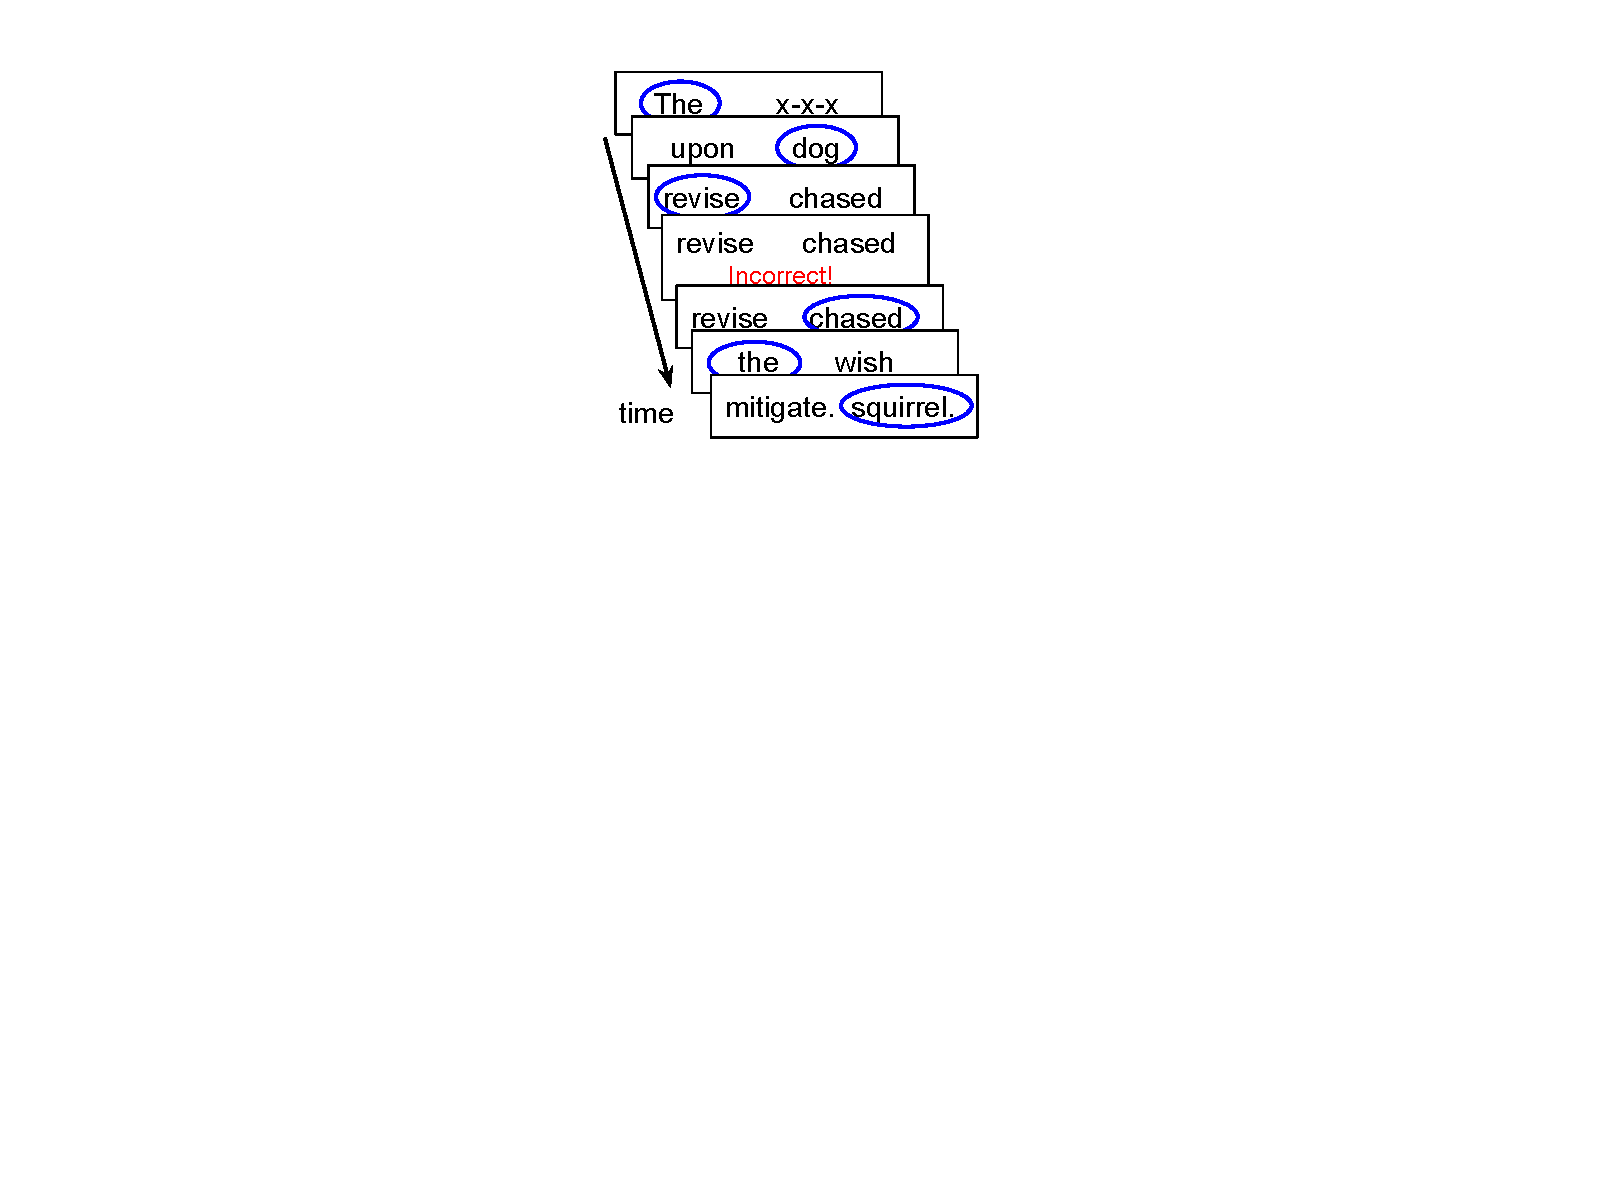
\includegraphics[clip, trim=9cm 12.5cm 10cm 1cm,width=.8\textwidth]{maze_diagram.pdf}\\} 
		\begin{small}
			Participants see two words at a time and try to select the correct word.  When the participant makes a mistake, they must correct it to continue. Blue circles indicate selected words.
			
		\end{small}
		
	\end{minipage}
	~~~
	\begin{minipage}{.5\textwidth}	
				\captionof{figure}{Accuracy versus RT}
		{\center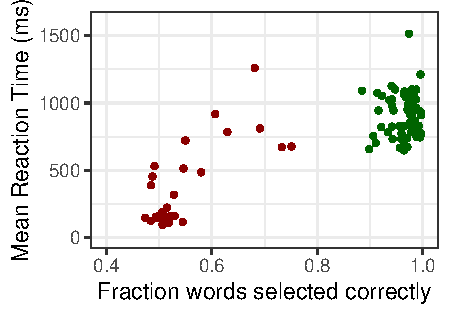
\includegraphics[width=\textwidth]{error.pdf}\\} 
		\begin{small}
			Correlation between participant's accuracy on the Maze task and RT. Participants with less than 80\% accuracy (in red) were excluded from analyses. 
			
		\end{small}
	\end{minipage}
\end{figure}
\vspace{1em}
\begin{figure}
		\begin{minipage}{.5\textwidth}
		\captionof{figure}{Surprisal and RT\\
		}
		{\center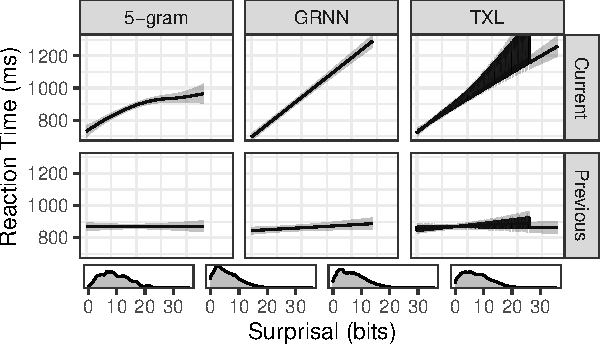
\includegraphics[width=\textwidth]{gam.pdf}\\} 
		\begin{small}
			Current word surprisal is linearly predictive of RT, but previous word surprisal is not predictive of RT.
			
		\end{small}
	\end{minipage}	
	~~~
\begin{minipage}{.5\textwidth}
	\captionof{figure}{Comprehension question accuracy}
	{\center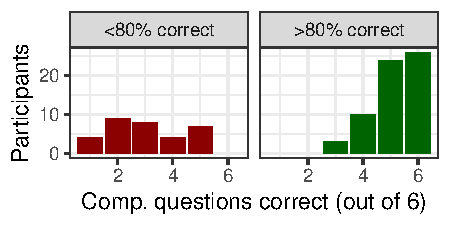
\includegraphics[width=\textwidth]{comp.pdf}\\} 
	\begin{small}
		Participants with higher accuracy on the Maze task also did better on comprehension questions. 
		
	\end{small}
\end{minipage}
	
\end{figure}

	\setlength{\tabcolsep}{4pt}
		\captionof{table}{Regression Coefficients}
\begin{small}%TODO do I even include p-values??
%\centering
\begin{tabular}{l|rlr|rlr|rlr}
	\hline
	&\multicolumn{3}{c|}{5-gram}&\multicolumn{3}{c|}{GRNN}&\multicolumn{3}{c}{TXL}\\
		 & Est & CI & $p$ & Est & CI & $p$ &Est & CI & $p$ \\ 
		 \hline
Intercept & 867.7 & [829.6, 904.3] & 0.00 & 868.5 & [835.4, 903] & 0.00 & 866.5 & [830.4, 900.7] & 0.00 \\
Surprisal & 10.6 & [8.6, 12.6] & 0.00 & 22.1 & [19.8, 24.4] & 0.00 & 17.0 & [14.8, 19.2] & 0.00 \\
Frequency & -4.2 & [-7.3, -0.9] & 0.01 & 1.7 & [-1.2, 4.6] & 0.25 & -0.8 & [-3.7, 2.2] & 0.59 \\ 
Length & 20.1 & [15.3, 24.7] & 0.00 & 18.0 & [13.6, 22.4] & 0.00 & 20.8 & [16.4, 25.3] & 0.00 \\ 
Freq : Length & 1.1 & [0.4, 1.8] & 0.00 & 1.2 & [0.4, 1.9] & 0.00 & 1.2 & [0.5, 2] & 0.00 \\ 
\hline
Past Surprisal & 1.9 & [0.3, 3.4] & 0.02 & 1.9 & [0.6, 3.3] & 0.01 & 0.1 & [-1.2, 1.3] & 0.95 \\ 
Past Freq & 3.0 & [0.8, 5.2] & 0.01 & 1.5 & [-0.2, 3.3] & 0.09 & 0.9 & [-0.9, 2.8] & 0.35 \\ 
Past Length & -5.0 & [-8.7, -1.5] & 0.01 & -6.9 & [-10.5, -3.3] & 0.00 & -5.3 & [-9, -1.7] & 0.00 \\ 
Past Freq : Length& -1.0 & [-1.7, -0.3] & 0.01 & -1.3 & [-1.9, -0.6] & 0.00 & -1.2 & [-1.9, -0.5] & 0.00 \\ 
\hline
\end{tabular}
\vspace{.5em}

\end{small}
		\begin{small}
			Point estimates, credible intervals, and p-value equivalents. Models were run with centered predictors and full mixed effects by subject. Surprisal is in bits, frequency is in $log_2$ occurances per billion words. 
		\end{small}
\vspace{.5em}

	\begin{small}{
			\noindent\textbf{References:}
			Boyce et al (2020). \textit{J Mem. Lang.} $\bullet$
			Dai et al (2019) arXiv:1901.02860 $\bullet$
			Forster et al (2009). \textit{Behav. Res. Methods} $\bullet$
			Futrell et al (2017). arXiv:1708.05763 $\bullet$
			Gulordava et al (2018).  \textit{NAACL-HLT 2018} $\bullet$
			Sloggett et al (2020). \textit{CUNY 2020} $\bullet$
			Witzel et al (2012).  \textit{J Psycholinguist Res} 
			%TODO add cites for length, freq, surprisal justification
		}
	\end{small}

\end{document}
